\documentclass{uws_learning_guide}

\usepackage{amsmath}
\usepackage{amssymb}
\usepackage{booktabs}
\usepackage{longtable}
\usepackage{enumerate}

% Setup unit information
\unitnumber{300958}
\unitname{Social Web Analytics}
\unitlevel{3}
\teachingsession{Spring}
\teachingyear{2014}
\unitimage{768px-Internet_map_crop}

% set up holdays dates
\newcommand{\teachingsessiondate}{28th of July}
\newcommand{\intersessionbreak}{22nd of September}
\newcommand{\goodfridaydate}{18th of April}
\newcommand{\goodfridayweek}{8}
\newcommand{\eastermondaydate}{21st of April}
\newcommand{\eastermondayweek}{9}
\newcommand{\anzacdaydate}{25th of April}
\newcommand{\anzacdayweek}{9}
\newcommand{\labourdaydate}{6th of October}
\newcommand{\labourdayweek}{11}

% \newcommand{\publicholidays}{
% There are three public holidays
% this semester Good Friday (\goodfridaydate{} \printteachingyear{}, during week
% \goodfridayweek), Easter Monday (\eastermondaydate~\printteachingyear{},
% during week \eastermondayweek), and Anzac Day
% (\anzacdaydate~\printteachingyear{}, during week \anzacdayweek).}
\newcommand{\publicholidays}{
There is one public holiday
this semester, Labour Day (\labourdaydate~\teachingyear, during week
\labourdayweek).}

\newcommand{\timetablelink}{\url{http://platformweb.uws.edu.au/pweb_tt/start.asp}}


\DeclareMathOperator{\var}{Var}

\newcommand{\vuws}{$\nu$UWS}

\begin{document}

\pagenumbering{roman}

\lgtitlepage

%% set spacing to make guide less cluttered
\onehalfspacing

\lgkey



\begin{tabularx}{\textwidth}{|>{\columncolor{tableshade}}p{3cm}|X|}
\hline
\rowcolor{tableshade}
\multicolumn{2}{|l|}{\texttitle{\hintlogo{} STAFF}} \\
\hline
\texttitle{Unit Coordinator} &
\setlength{\parskip}{\medskipamount}
Dr Laurence Park\newline
EN.1.32 Parramatta South\newline
Phone: 9685 9065 \hfill
Email: lapark@scem.uws.edu.au\newline
Consultation times to be announced on \vuws{} \\
\hline
%\texttitle{Unit administration} & 
%<Insert name [If not applicable, delete unit administration section]>\newline
%<Insert location>\newline
%Phone: <Insert Phone number> \hfill
%Email: <Insert email> \\
%\hline
\texttitle{Teaching team} &
Assoc. Prof. Glenn Stone\newline
EN.1.31 Parramatta South\newline
Phone: 4620 3467 \hfill
Email: g.stone@uws.edu.au \newline
Consultation times to be announced on \vuws{} \\
\cline{2-2}
%& Dr Shatha Aziz\hfill Email: s.aziz@uws.edu.au\newline
%Consultation times to be announced on \vuws{} \\
& Don Shearman \hfill Email: d.shearman@uws.edu.au \\
& Consultation times to be announced on \vuws{} \\
\hline
\end{tabularx}

\begin{tabularx}{\textwidth}{|X|}
  \hline \rowcolor{tableshade}
  \texttitle{\informationlogo{} STUDENT FEEDBACK AND IMPROVEMENTS TO THE UNIT} \\
  \hline \setlength{\parskip}{\medskipamount} Student feedback pays a
  vital role in improving the quality and educational effectiveness of
  UWS units and in ensuring academic staff keep in touch with student
  needs. You are welcome to provide feedback that is related to the
  teaching of this unit. At the end of the semester you will be given
  the opportunity to complete a Student Feedback on Unit (SFU)
  questionnaire to assess the unit. If requested by your unit
  coordinator, you may also have the opportunity to complete a Student
  Feedback on Teaching (SFT) questionnaire to provide feedback for
  individual teaching staff.

  As a result of student feedback, the following changes and
  improvements have recently been made:
  \begin{itemize}
  \item All lectures are recorded.
  \item Students are assessed on five of the eight weekly tests.
  \end{itemize} \\
  \hline
\end{tabularx}

\newpage

\tableofcontents

\newpage

\setcounter{page}{1}    % set page to 1 again to start arabic count
\pagenumbering{arabic}


\section{About \printunitname}

\subsection{An introduction to this unit}

%<Insert description from approved unit template/handbook>

The Social Web provides everyone with an elegant platform to voice
their opinion. The rapid take up of Web based social networking tools
by society has lead to an abundance of data containing the opinions of
millions of individuals.  Therefore, the analysis of information from
Facebook, Twitter and Google+ should allow us to identify trends and
relationships in society. Whilst this has interest on a personal
level, the killer­app will be in analysing such data for business;
tracking the buzz around a new product, understanding the links
between customers etc. This unit will introduce its students to the
Social Web data that is available, and blend computational,
mathematical and statistical concepts to allow extraction and analysis
of such data.

This Level 3 unit introduces students to various mathematical and
statistical techniques supporting the study of computing, engineering
and science. Presentation of the content will emphasise the correct
principles and procedures for accessing social Web data, performing
and understanding exposure analysis, analysing and visualising social
relationships using graphs, identifying important information using
text mining, and investigating the significance of trends. Topics
include graph analysis, text mining, temporal and spatial analysis,
and exposure analysis.


\printunitname{} is a core unit within the Bachelor of Information and
Communications Technology. 

Thus unit has the following prerequisites:
\begin{itemize}
\item 300700 Statistical Decision Making
\end{itemize}



\subsection{Textbook}

% <Insert required text book/s>

There is no official text book for this Unit. We have compiled an
online book that covers the topics in this Unit:
\begin{itemize}
\item \url{http://en.wikipedia.org/wiki/User:Lapark/Books/swa}
\end{itemize}



\subsection{Unit learning outcomes}

%<Insert brief information about major focus of unit learning outcomes>

Students are expected to gain an understanding of the fundamental
concepts of Web social networks as well as the ability to apply modern
mathematical and statistical techniques to analyse the social network
properties.  On successful completion of this unit, students will be
able to:

\begin{enumerate}
\item Extract and process structured data from social Web sources.
\item Use mathematical and statistical methods to identify significant
  trends though time and space in the social Web.
\item Use computer algorithms to visualise complex social Web
  interactions.
\item Design and implement a simple text search engine.
\item Construct clustering and classification models on text.
\item Represent and analyse data in graphs using graph statistics and
  random walk analysis.
\item Use mathematical and statistical techniques to identify critical
  regions of a social network.
\end{enumerate}

Each of the assessment tasks has been designed to evaluate the extent
to which you have achieved these learning outcomes.


\subsection{Approach to learning}

%<Insert information on various types of learning activities
%e.g. lectures, practicals, workshops, industry visits
%etc. highlighting the activity of major focus>

This unit will be offered on the Parramatta, Kingswood and
Campbelltown campuses over a twelve week period.  Each week will
consist of a two hour lecture and a two hour computer lab class.


%<Insert information on how learning activities support the attainment
%of learning outcomes >

There will be eight quizzes, a group project and a final examination in this
offering.  The project and tests are designed to gauge your
achievement and performance in relation to the unit learning outcomes.
These quizzes and the group project are also excellent preparation for the final
examination, which is a summative examination.

%<Insert information on approach to Blended Learning e.g. how online
%and face-to-face activities integrate and support each other. >

Due to the multi-campus nature of the unit, the lectures will be
presented as a campus tour, where the face-to-face lecture will be
delivered on one campus and can be viewed online by students not
attending the chosen campus. The campus chosen for the face-to-face
lecture will be set according to the tour schedule presented in \vuws{}.
All of the unit material will be released on \vuws{} as the semester
progresses.  The lectures from each campus will be recorded and
uploaded to \vuws{}.  These online resources should be used as a good
source of revision and should not replace the face to face time during
the weekly lectures and lab classes.

\subsection{Contribution to Course Learning Outcomes (CLOs)}

%<Insert information on the courses that this unit is taught into and
%how unit learning outcomes relate to course learning outcomes. ****
%Sample text below****>

This is a third level core unit in the Bachelor of Information and
Communications Technology. This unit is responsible for developing the
fundamental data analysis skills required for examining data found in
social networks (text, graphs, spatial and temporal data).
 




% \begin{landscape}
% {\huge <Insert Course Name Here>}
% \vspace{1cm}
% \hrule
% \vspace{-0.21cm}
% \begin{tabularx}{\textwidth}{|>{\columncolor{tableshade}}p{1.cm}|p{6.45cm}|p{1.3cm}|p{1.3cm}|p{1.3cm}|p{1.3cm}|p{1.3cm}|p{1.3cm}|p{1.3cm}|p{1.3cm}|p{1.3cm}|p{1.3cm}|}
% \rowcolor{tableshade}
% %\multicolumn{5}{|l|} \\

% %%%%%%%%%%%%%%%%%%%%%%%%%%%%%%%%%%%%%%%%%%%%%%%%%%%%%%%%%%%%%%%%%
% 																								%%%%
% 																								%%%%
% \texttitle{CLO \newline Number}
% & \center{\texttitle{<Insert stem sentence that goes with \newline the CLO statements below>}} 
% & \center{\texttitle{ULO 1}} 
% & \center{\texttitle{ULO 2}} 
% & \center{\texttitle{ULO 3}} 																							% 	MATHS UNITS DO NOT NEED TO FILL IN THIS CLO TABLE. IF YOU ARE FILLING OUT THIS TEMPLATE FOR A MATHS UNIT, COMMENT	
% & \center{\texttitle{ULO 4}} 																							%	OUT THE ENTIRE LANDSCAPE PAGE.
% & \center{\texttitle{ULO 5}} 
% & \center{\texttitle{ULO 6}} 
% & \center{\texttitle{ULO 7}} 
% & \center{\texttitle{ULO 8}}
% & \center{\texttitle{ULO 9}} 
% & {\center \texttitle{ULO 10}}  \\
% \cline{1-12}	 	
% 																								%%%%
% 																								%%%%
% %%%%%%%%%%%%%%%%%%%%%%%%%%%%%%%%%%%%%%%%%%%%%%%%%%%%%%%%%%%%%%%%%


% %%%%%%%%%%%%%%%%%%%%%%%%%%%%%%%%%%%%%%%%%%%%%%%%%%%%%%%%%%%%%%%%%
% 																								%%%%
% 																								%%%%
% \texttitle{1}
% & \center{\texttitle{<Insert CLO statement>}} 																				% PLEASE INSERT A COMPLETE LIST OF CLOs FROM THE RELEVANT COURSE DOCUMENT

% & \center{\texttitle{Enter Item}} 																						% CHOOSE BETWEEN 'INTRODUCE", "DEVELOP" OR "ASSURE" TO INDICATE CONTRIBUTION OF YOUR ULO TOWARDS ATTAINMENT OF THE CLO, 																											
% & \center{\texttitle{Enter Item}} 																						% OR ENTER "X" IF YOU ARE NOT SURE ABOUT THE THREE ASSURANCE LEVELS. 
% & \center{\texttitle{Enter Item}} 																						% LEAVE THE CELL BLANK WHEN THE ULO IS NOT MAPPED TO A CLO.
% & \center{\texttitle{Enter Item}} 																						% IT IS RECOMMENDED THAT NO MORE THAN 3 CLOs BE SELECTED FOR EACH ULO. 
% & \center{\texttitle{Enter Item}} 																						% IT IS NOT NECESSARY THAT EACH ULO IS MAPPED TO A CLO AND NOT ALL CLOs NEED TO BE ADDRESSED IN EVERY UNIT
% & \center{\texttitle{Enter Item}} 
% & \center{\texttitle{Enter Item}}
% & \center{\texttitle{Enter Item}} 
% & \center{\texttitle{Enter Item}} 
% & {\center \texttitle{Enter Item}}  \\
% \cline{1-12}
% 																								%%%%
% 																								%%%%
% %%%%%%%%%%%%%%%%%%%%%%%%%%%%%%%%%%%%%%%%%%%%%%%%%%%%%%%%%%%%%%%%%

% %%%%%%%%%%%%%%%%%%%%%%%%%%%%%%%%%%%%%%%%%%%%%%%%%%%%%%%%%%%%%%%%%
% 																								%%%%
% 																								%%%%
% \texttitle{2}
% & \center{\texttitle{<Insert CLO statement>}} 																				% PLEASE INSERT A COMPLETE LIST OF CLOs FROM THE RELEVANT COURSE DOCUMENT

% & \center{\texttitle{Enter Item}} 																						% CHOOSE BETWEEN 'INTRODUCE", "DEVELOP" OR "ASSURE" TO INDICATE CONTRIBUTION OF YOUR ULO TOWARDS ATTAINMENT OF THE CLO, 																											
% & \center{\texttitle{Enter Item}} 																						% OR ENTER "X" IF YOU ARE NOT SURE ABOUT THE THREE ASSURANCE LEVELS. 
% & \center{\texttitle{Enter Item}} 																						% LEAVE THE CELL BLANK WHEN THE ULO IS NOT MAPPED TO A CLO.
% & \center{\texttitle{Enter Item}} 																						% IT IS RECOMMENDED THAT NO MORE THAN 3 CLOs BE SELECTED FOR EACH ULO. 
% & \center{\texttitle{Enter Item}} 																						% IT IS NOT NECESSARY THAT EACH ULO IS MAPPED TO A CLO AND NOT ALL CLOs NEED TO BE ADDRESSED IN EVERY UNIT
% & \center{\texttitle{Enter Item}} 
% & \center{\texttitle{Enter Item}}
% & \center{\texttitle{Enter Item}} 
% & \center{\texttitle{Enter Item}} 
% & {\center \texttitle{Enter Item}}  \\
% \cline{1-12}	 	
% 																								%%%%
% 																								%%%%
% %%%%%%%%%%%%%%%%%%%%%%%%%%%%%%%%%%%%%%%%%%%%%%%%%%%%%%%%%%%%%%%%%
% \end{tabularx} 

% \vspace{4cm}


% {\huge <Insert Course Name Here>}

% \vspace{1cm}
% \hrule
% \vspace{-0.21cm}
% \begin{tabularx}{\textwidth}{|>{\columncolor{tableshade}}p{1.cm}|p{6.45cm}|p{1.3cm}|p{1.3cm}|p{1.3cm}|p{1.3cm}|p{1.3cm}|p{1.3cm}|p{1.3cm}|p{1.3cm}|p{1.3cm}|p{1.3cm}|}
% \rowcolor{tableshade}
% %\multicolumn{5}{|l|} \\
% \texttitle{CLO \newline Number}
% & \center{\texttitle{<Insert stem sentence that goes with \newline the CLO statements below>}} 
% & \center{\texttitle{ULO 1}} 
% & \center{\texttitle{ULO 2}} 
% & \center{\texttitle{ULO 3}} 
% & \center{\texttitle{ULO 4}} 
% & \center{\texttitle{ULO 5}} 
% & \center{\texttitle{ULO 6}} 
% & \center{\texttitle{ULO 7}} 
% & \center{\texttitle{ULO 8}}
% & \center{\texttitle{ULO 9}} 
% & {\center \texttitle{ULO 10}}  \\
% \cline{1-12}	 	

% \texttitle{1}
% & \center{\texttitle{<Insert CLO statement>}} 
% & \center{\texttitle{Enter Item}} 
% & \center{\texttitle{Enter Item}} 
% & \center{\texttitle{Enter Item}} 
% & \center{\texttitle{Enter Item}} 
% & \center{\texttitle{Enter Item}} 
% & \center{\texttitle{Enter Item}} 
% & \center{\texttitle{Enter Item}}
% & \center{\texttitle{Enter Item}} 
% & \center{\texttitle{Enter Item}} 
% & {\center \texttitle{Enter Item}}  \\
% \cline{1-12}	 	

% \texttitle{2}
% & \center{\texttitle{<Insert CLO statement>}} 
% & \center{\texttitle{Enter Item}} 
% & \center{\texttitle{Enter Item}} 
% & \center{\texttitle{Enter Item}} 
% & \center{\texttitle{Enter Item}} 
% & \center{\texttitle{Enter Item}} 
% & \center{\texttitle{Enter Item}} 
% & \center{\texttitle{Enter Item}}
% & \center{\texttitle{Enter Item}} 
% & \center{\texttitle{Enter Item}} 
% & {\center \texttitle{Enter Item}}  \\
% \cline{1-12}	 	
% \end{tabularx} 
% \end{landscape}

\section{Assessment details}

\subsection{Assessment summary}


There are seven main assessment activities in this unit:
\begin{center}
\begin{tabularx}{\textwidth}{|>{\raggedright\columncolor{tableshade}}p{1.5cm}|>{\raggedright\let\\\tabularnewline}X|>{\raggedright\let\\\tabularnewline}p{4cm}|>{\raggedright\let\\\tabularnewline}p{1.5cm}|}
  \hline
  \rowcolor{tableshade}
  \texttitle{Assessment Number} & \texttitle{Assessment item and due date} & \texttitle{Learning Outcomes} & \texttitle{Value (/100)} \\
  \hline
  1. & Online quizzes 1-8 & 1,2,3,4,5,6,7 & $\text{20}^{\star}$ \\
  2. & Project           & 1,2,3,4,5,6,7 & 30 \\
  3. & Final Examination & 1,2,3,4,5,6,7 & 50 \\
  \hline
\end{tabularx}
\end{center}
\textbf{$\star$ Each quiz is marked out of 4. The highest 5 marks from
  the 8 online quizzes will be taken.}

The compulsory assessment tasks are: participation in the final
examination. See below for further details. Students who do not
participate in this task will receive an automatic failing grade
(AF).
\begin{itemize}
\item An \textbf{absent fail}, AF grade is defined as: Student has not
officially withdrawn from the unit and has failed to complete one or
more of the compulsory assessment requirements for the unit.

\item A \textbf{compulsory fail}, CF grade is defined as: A student has
failed a compulsory component of a unit. If a student receives a CF
grade, they have failed the unit irrespective of the percentage mark
achieved.
\end{itemize}

\subsection{Calculation of Final Mark and Grade}

Marks and subsequent grades for \printunitnumber{} \printunitname{} will be
calculated in the following way:
\begin{itemize}
\item
  Quizzes (20\%) + Group project (30\%) + Final Examination (50\%)
\end{itemize}

To pass this unit, you must:
\begin{enumerate}
\item Obtain at least 40\% for the Final Exam.
\item Obtain at least 50\% overall.
\end{enumerate}

The following cut-off marks may act as a guide to the final grade awarded:
\begin{itemize}
\item High Distinction (H):            85/100 or higher
\item Distinction (D):                 75/100 - 84/100
\item Credit (C):                      65/100 - 74/100
\item Pass (P):                        50/100 - 64/100
\end{itemize}
In this unit learning and teaching activities consist of a weekly
two-hour lecture and a weekly two-hour computer lab. The computer lab
is designed to allow student to implement the ideas presented in the
lectures.


Students are expected to work individually through the set topics,
receiving assistance as required and attempting specific lab
tasks for each topic. Students should be aware that in this unit,
later topics build on the material covered earlier.



\subsection{\hintlogo{}  Feedback on assessment}

Feedback is an important part of the learning process that can improve
your progress towards achieving the learning outcomes.  Feedback is
any written or spoken response made in relation to academic work such
as an assessment task, a performance or product.  It can be given to
you by a teacher, an external assessor or student peer and may be
given to individually or to a group of students.  As a UWS student, it
is your responsibility to seek out and act on feedback that is
provided to you as a resource to further your learning.

In this unit you can expect automatic feedback on your weekly quizzes,
and written feedback for the group project.
You are also
welcome to email the unit coordinator, Dr Laurence Park
(lapark@scem.uws.edu.au) to discuss your progress.

\subsection{Assessment 1: Online Quizzes, best 5 of 8 @ 4\% (20\%)}

\subsubsection{Overview}

The quizzes will address learning outcomes 1, 2, 3, 4, 5, 6, and 7.

\subsubsection{Details}

The online quizzes will be short tests, expected to take 15 minutes
each, that will provide students a chance to assess their knowledge
throughout the unit.  There will be eight quizzes, but only the best
five of the eight will contribute towards the students final grade.


\subsection{Assessment 2: Group Project, weighting 30\%}

\subsubsection{Overview}

The group project will address learning outcomes 1, 2, 3, 4, 5, 6, and 7.

\subsubsection{Details}

The group project is designed to examine if each student can apply the
knowledge from the unit to analyse a social network.  The project
will be completed with a group of students, therefore it is crucial
that all students in the team work together and delegate the tasks
effectively.

More information on this may be found on the \vuws~site.


\subsection{Assessment 3: Final Exam (50\%)}

\subsubsection{Overview}

The project will address learning outcomes 1, 2, 3, 4, 5, 6, and 7.

\subsubsection{Details}

This is a compulsory assessment item. Students who do not attempt the
final (or deferred exam, if eligible) will be given an automatic
failing grade.  Students who fail to pass the 40\% hurdle on this exam
will receive a compulsory fail grade.

This is an open book examination to determine whether you are able to
employ the appropriate mathematical and statistical methods and
techniques in given situations. It will be 2 hours in duration.




\subsection{\hintlogo{} Annotated exemplars and standards}

The following are typical questions found in an exam for this
unit. The number of marks associated to each question reflect the
difficulty of each question.


\subsubsection*{Question (4 marks)}

Plot the degree distribution of the following graph and identify if it
is a small world graph or not.
% g = barabasi.game(10, directed=FALSE)
% plot(g)
% table(degree(g))

\vspace{-6em}
\begin{center}
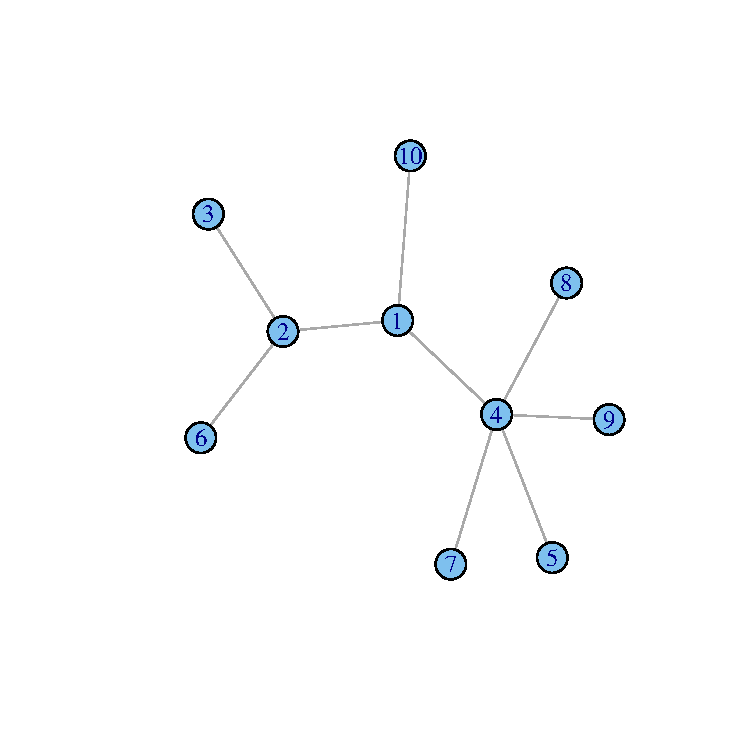
\includegraphics{bnetwork}
\end{center}

\vspace{-14em}
\subsubsection*{Solution}

The degree distribution is:
\begin{center}
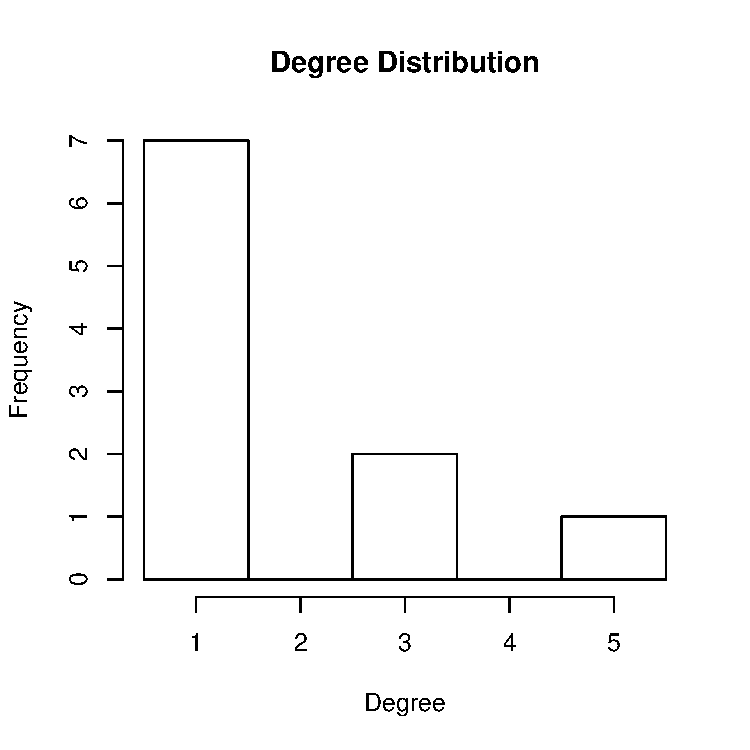
\includegraphics[scale=0.7]{bnetwork-dist}
\end{center}

The distribution shows that the frequency is exponentially decreasing
as the degree increases and so this graph resembles a small world
graph.


\subsubsection*{Question (4 marks)}

Using the following document set:
\begin{enumerate}
\item One one was a race horse.
\item Two two was one too.
\item One one won one race.
\item Two two won one too.
\end{enumerate}
Complete the following tasks:
\begin{enumerate}
\item Construct a term frequency matrix of the following document set.
\item Compute the term weight of each term.
\item Order the words from most important to least important.
\end{enumerate}
Note: use the stop word list \{was, a, too\}.

\subsubsection*{Solution}

After removing the stop words and case folding, the term frequency matrix is:
\begin{center}
\begin{tabular}{lcccccc}
\toprule
  & one & race & horse & two & won \\
\midrule
1 & 2 & 1 & 1 & 0 & 0 \\
2 & 1 & 0 & 0 & 2 & 0 \\
3 & 3 & 1 & 0 & 0 & 2 \\
4 & 1 & 0 & 0 & 2 & 1 \\
\bottomrule
\end{tabular}
\end{center}
The term weight of each word is calculated using:
\begin{align*}
  w_t = \log{\left (\frac{N}{f_t}\right )}
\end{align*}
where $N = 4$.
\begin{center}
\begin{tabular}{lccccc}
\toprule
  & one & race & horse & two & won \\
\midrule
$f_t$ & 4 & 2 & 1 & 2 & 2 \\
$w_t$ & 0 & 0.693 & 1.386 & 0.693 & 0.693 \\
\bottomrule
\end{tabular}
\end{center}
Therefore the order of the words, from most important to least important is:
\begin{enumerate}
\item horse
\item race 
\item two 
\item won 
\item one
\end{enumerate}


\subsubsection*{Question (4 marks)}

Arrange the set of words into two clusters using single linkage clustering from the following adjacency matrix:
\begin{center}
\begin{tabular}{lccccc}
\toprule
  & one & race & horse & two & won \\
\midrule
one   & 0 & 1 & 1 & 2 & 2 \\
race  & 1 & 0 & 1 & 3 & 2 \\
horse & 1 & 1 & 0 & 3 & 1 \\
two   & 2 & 3 & 3 & 0 & 1 \\
won   & 2 & 2 & 1 & 1 & 0 \\
\bottomrule
\end{tabular}
\end{center}

We choose ``one'' and ``race'' as the most similar pair of clusters, and merge them to obtain:
\begin{center}
\begin{tabular}{lcccc}
\toprule
  & one-race & horse & two & won \\
\midrule
one-race  & 0 & 1 & 2 & 2 \\
horse     & 1 & 0 & 3 & 1 \\
two       & 2 & 3 & 0 & 1 \\
won       & 2 & 1 & 1 & 0 \\
\bottomrule
\end{tabular}
\end{center}

We choose ``one-race'' and ``horse'' as the next most similar pair of clusters, and merge them to obtain:
\begin{center}
\begin{tabular}{lccc}
\toprule
  & one-race-horse & two & won \\
\midrule
one-race  & 0 & 2 & 1 \\
two       & 2 & 0 & 1 \\
won       & 1 & 1 & 0 \\
\bottomrule
\end{tabular}
\end{center}

We choose ``two'' and ``won'' as the next most similar pair of clusters, and merge them to obtain:
\begin{center}
\begin{tabular}{lcc}
\toprule
  & one-race-horse & two-won \\
\midrule
one-race-horse  & 0 & 1 \\
two-won         & 1 & 0 \\
\bottomrule
\end{tabular}
\end{center}

This gives us the two clusters: \{one, race, horse\} and \{two, won\}.

\subsubsection*{Question (10 marks)}

The table below shows the counts of all time \emph{likes} by age group and gender for a particular facebook page.

\begin{center}
\begin{tabular}{rrrrrrrr}
  \toprule
 & 13--17 & 18--24 & 25--34 & 35--44 & 45--54 & 55--65 & 65+ \\ 
  \midrule
F & 0 & 16 & 9 & 7 & 3 & 1 & 1 \\ 
  M & 3 & 99 & 30 & 6 & 3 & 1 & 3 \\ 
   \bottomrule
\end{tabular}
\end{center}

The owner of this page is interested in determining whether the age profile of likes depends on gender.

\begin{enumerate}[i)]
\item State the \emph{null} hypothesis for the statistical test that corresponds to the question, ``Does the age profile of likes depends on gender?''
\item Identify one problem with using a $\chi^2$ (Chi-squared) test with this data.
\item Using only the age groups 18--24 , 25--34  and 35--44, find the proportion of likes in each age group.
\item Using only the same age groups,  find the proportion of likes in each gender.
\item Using only the same age groups,  calculate a $\chi^2$ statistic for testing whether the age
  profile varies by gender, and state its degrees of freedom.
\end{enumerate}

{\bf Solution}

\begin{enumerate}[i)]
\item The null hypothesis would be 

\begin{quote}
$H_0$: Age and Gender are INDEPENDENT
\end{quote}
\item Several of the cells have very small counts, and therefore the
  $\chi^2$ approximation will not be accurate.
\item Using only the sub-table
\begin{center}
\begin{tabular}{rrrr}
  \toprule
 & 18-24 & 25-34 & 35-44 \\ 
  \midrule
F & 16 & 9 & 7 \\ 
  M & 99 & 30 & 6 \\ 
   \bottomrule
\end{tabular}
\end{center}
Total number of likes is 167. Therefore proportions are ``18-24''
(99+16)/167 = 0.689, ``25-34'' (9+30)/167 = 0.234, ``35-44''
(7+6)/167 = 0.078
\item ``F''  (16+9+7)/167 = 0.192, ``M'' (99+30+6)/167 = 0.808
\item \[
\chi^2 = \sum \frac{(O_{ij}-E_{ij})^2}{E_{ij}}\]

Expected counts are $E_{ij} = n\times p_i \times q_j$
\begin{center}
\begin{tabular}{rrrr}
  \toprule
 & 18-24 & 25-34 & 35-44 \\ 
  \midrule
F & 22.09 & 7.50 & 2.50 \\ 
  M & 92.97 & 31.58 & 10.53 \\ 
   \bottomrule
\end{tabular}
\end{center}

Therefore, $\chi^2 = 12.50$. There are 2 degrees of freedom
($(r-1)\times (c-1)$).
\end{enumerate}

\subsubsection*{Question (10 marks)}

\begin{enumerate}[a)]
\item Explain the main features of BACI designs and when they might be
  used.
\item A mobile phone company which is about to start a major
  advertising campaign collects information about mentions
  on Twitter. Using a search the company collects the number of
  mentions of their product for 3 days before the campaign and 3 days
  after the campaign. They also collect the number of mentions for
  their main competitor on the same days. The data are below.

\begin{center}
\begin{tabular}{rrr}
\toprule
&\multicolumn{2}{c}{Advertising}\\
\cmidrule(r){2-3}
&Before&After\\
\midrule
Company&105, 107,  98& 110, 139, 120\\
Competitor&82, 100,  80&  88,  89,  78\\ 
\bottomrule
\end{tabular}
\end{center}

\begin{enumerate}[i)]
\item Calculate the total mentions for each company before and after
  the advertising.
\item Calculate the \emph{contrast} for the interaction between
  company and time.
\item Calculate the \emph{Sum of Squares} for the interaction between
  company and time.
\item Given that the sum of squares for error is 795.3, find the
  $F$-statistic for the interaction between
  company and time.
\end{enumerate}
\end{enumerate}

\textbf{Solution}
\begin{enumerate}[a)]
\item A BACI (or Before/After/Control/Impact) design is used to
  test the impact of an intervention. The key features are that the
  results before and after an intervention are compared to a control
  that should not be directly affected by the intervention.
\item \begin{enumerate}[i)]
\item \begin{tabular}{rrr}
  \toprule
 & Before & After \\ 
  \midrule
Company & 310 & 369 \\ 
  Competitor & 262 & 255 \\ 
   \bottomrule
\end{tabular}
\item Contrast for the interaction is (310+255) - (262+369) = -66
\item SSQ = $\frac{\text{contrast}^2}{4n}$ = $\frac{66^2}{12}$ = 363
\item $F = \frac{SSQ}{SSE/df_E} = \frac{363}{795.3/8} = 3.651$
\end{enumerate}
\end{enumerate}






















\subsection{Marking criteria and standards}

Your total mark for the unit is the weighted sum of all your
assessment marks.  Your final grade for the unit is determined by the
percentage of the total mark you achieve, according to the following
key:

\begin{center}
  \begin{tabularx}{0.5\textwidth}{XX}
    \toprule
    Percentage of marks & Grade \\
    \midrule
    100\% - 85\% & H (High Distinction) \\
    84\% - 75\% & D (Distinction) \\
    74\% - 65\% & C (Credit) \\
    64\% - 50\% & P (Pass) \\
    49\% - 0\% & F Fail \\
    \bottomrule
  \end{tabularx}
\end{center}

An exception to this rule is anyone who fails to pass the Final Exam
hurdle, but has obtained a weighted sum of greater than or equal to
50\%, will receive a grade of CF (compulsory fail).

\subsection{General Assessment Requirements}

\subsubsection{\informationlogo{} Assignment cover sheet}

All assignments are to be submitted with a signed Assignment Cover
Sheet. Assignment cover sheets may be found on \vuws{}.

\subsubsection{Late submission or missed attempt}

A student who submits a late assessment without approval for an
extension will be penalised by 10 per cent per calendar day up to 10
days, i.e. marks equal to 10 per cent of the assessment’s worth will
be deducted as a `flat rate' from the mark awarded. For example, for
an assessment that has a possible highest mark of 50, the student’s
awarded mark may have five marks deducted for each late day. Saturday
and Sunday count as one day each. Assessments will not be accepted
after the marked assessment task has been returned to students who
submitted the task by the due.  


\subsubsection{Extension of due date for submission}

Normally no extension will be approved. Contact the unit coordinator
before the due date of the assignment for any extension in
extraordinary circumstances only.

Where special consideration is sought for circumstances involving more
than three consecutive days or more than five days within a teaching
period, students should complete a Special Consideration Application,
available from the \vuws{} website: \href{http://www.uws.edu.au/currentstudents/current_students/getting_help/special_consideration2}{http://www.uws.edu.au/currentstudents/current\_students/getting\_help/special\_consideration2}



\section{Schedule of teaching activities}

%\rhead{Autumn}

The \printteachingsession{} teaching session begins on \teachingsessiondate{}
\printteachingyear{}.  The inter-session break begins on
\intersessionbreak{} \printteachingyear{}.  \publicholidays{}
When classes
fall on public holidays, students are expected to revise the missed
material in their own time. In the case of a missed lecture, lectures
online will be available within \vuws{}.

\noindent
%\renewcommand{\arraystretch}{1.3}
\begin{longtable}{|>{\columncolor{tableshade}}c|>{\raggedright}p{0.5\textwidth}|>{\raggedright}p{0.2\textwidth}|>{\raggedright\arraybackslash}p{0.15\textwidth}|}
\hline
\rowcolor{tableshade}
Week & Topic & Text readings & Assessment \\
\hline
1 & Introduction to the Social Web  & & \\
\hline
2 & Introductory R programming and data structures &  & \\
\hline
3 & Simple Exposure Analysis &  & \\
\hline
4 & Text Mining 1 (indexing, weighting, querying, metrics) &  & Online Test 1 \\
\hline
5 & Graphs 1 (Definition, Graph statistics, Storage) & &  Online Test 2 \\
\hline
6 & Visualisation &  &  Online Test 3 \\
\hline                                            
7 & Text Mining 2 (Clustering) &  &  Online Test 4 \\
\hline                                            
8 & Graphs 2 (PageRank, HITS, Shortest Path) &  & Online Test 5 \\
\hline
9 & Semester Break & &  \\
\hline                                             
10 & Time 1 (trends, trend periodicity)  & & Online Test 6 \\
\hline                                            
11 & Time 2 (BACI designs) &  & Online Test 7 \\
\hline
12 & Text Mining 3 (Sentiment Analysis) &  & Online Test 8  \\
\hline
13 & Spatial Analysis &  & Group Project Due \\
\hline                                            
14 & Revision &  & \\                
\hline
\end{longtable}


Each week, students are expected to attend lectures and
computer labs. For full details about the timetable for this unit, go to
\timetablelink{} and search for \printunitnumber{}.



\subsection*{Lectures}

Lectures are large classes where students are introduced to new ideas
and concepts. The notes presented in the lectures will be available in
the \printunitnumber{} \printunitname{} section of \vuws{}.

%\subsection*{Tutorials}
%
%Tutorials are small classes where students work through questions and
%problems related to the lecture content. It is expected that students
%attempt the tutorial questions before coming to the tutorials.

\subsection*{Computer Labs}

Computer Labs are small interactive classes based in a computer lab where
the tutor will discuss how to use computers to assist us in
solving statistical problems. Time will be given in the labs for
students to work on problems with the assistance of the tutor.


\section{Learning Resources}

\subsection{Overview of learning resources}

\begin{texttable}
\texttabletitle{RESOURCE}{HOW IT WILL ASSISST IN LEARNING}
\texttablerow{
  Teaching Team
}{
  Available for consultation.  Please email.
}
\texttablerow{
  Readings
}{
  Study relevant lecture notes, lab notes, and sections of the Wikipedia text book in addition to the sample papers.
}
\texttablerow{
  \vuws{}
}{
  All material relevant to this unit may be found on this site.  
}
\texttablerow{
  Library
}{
  Search Central is a great Library resource that will help you find information for this unit \href{http://library. uws.edu.au/}{http://library. uws.edu.au/}
}
\texttablerow{
  Participation in class
}{
To get the most from this unit, it is essential that each student participates in class. Participation includes asking questions, responding to questions and working through problems when they are given.
}
\end{texttable}





\subsection{{\Large \readinglogo{}} Recommended reading}

\begin{tabularx}{\textwidth}{|>{\raggedright\columncolor{tableshade}}p{3cm}|>{\raggedright\let\\\tabularnewline}X|}
%\begin{longtable}{|>{\raggedright\columncolor{tableshade}}p{3cm}|p{10cm}|}
  \hline
  \texttitle{Textbook} & There is no text book for this unit. \\
  \hline
 \texttitle{Additional reading list} &  
 The UWS library has the following books available for loan:
\href{http://readings.uws.edu.au/imageserver/readings.php?ci=6593}{http://readings.uws.edu.au/imageserver/readings.php?ci=6593}
 \\
 \hline
  \texttitle{Online resources} & 
  Wikipedia can be a great help with initial information on some topics. However in this unit Wikipedia articles should not be used in assessment tasks. \\
  \hline
  \texttitle{Literacy and/or numeracy resources} & 
  The Mathematics Education Support Hub (MESH) operates the online
  tutoring service - I Don’t Get it.
  (\href{http://www.uws.edu.au/mesh}{http://www.uws.edu.au/mesh}) over
  this Summer 3 period. \\
 \hline
\end{tabularx}
%\end{longtable}













\section{You and This Unit}

\subsection{\informationlogo{} What is expected of you}

\subsubsection{Credit points and Workload}
This unit is a 10 credit point unit and will require your full and
continuous attention to maintain the highest possible grades.  It is
expected that you will spend at least 10 hours each week (on average)
which includes the four (4) contact hours per week.  Some weeks you
will spend more time on learning activities and assessments and in
other weeks the workload will be somewhat less.  It will be essential
for you to keep up with the assigned reading so that you are properly
prepared for each session.

\subsubsection{Attendance}
Students are expected to attend the two hour lecture and a two
hour workshop each week.

\subsubsection{Online learning}
Students should access \vuws{} to obtain lecture notes and information,
and check their student email account at least twice a week.



\subsection{\warninglogo{} Student responsibilities and conduct}


\begin{texttable}
\texttablerow{Student responsibilities}{
  Familiarise yourself with University policies on assessment and
  examinations.

  Ensure that you understand the requirements, including timetables,
  for examinations and other assessments tasks.

  Ensure you read and understand the assessment requirements and note
  the submission dates, and seek assistance from the lecturer and/or
  unit coordinator when needed.

  Notify relevant staff (e.g. lecturer, unit coordinator, disability
  adviser) as soon as possible prior to, or at the beginning of, the
  semester to have special requirements accommodated.

  Submit your own individual and unassisted assessment work, except as
  otherwise permitted. Cheating, plagiarism, fabrication or
  falsification of data will be severely dealt with.

  Behave ethically and appropriately, avoiding any action or behaviour
  which would unfairly disadvantage or advantage another
  student. Where group work is assigned, ensure that every group
  member has the opportunity to contribute in a meaningful way to the
  assignment.  }

\texttablerow{Student conduct and behaviour}{
  Attend all lectures and lab classes – failure to attend is often the
  main cause for low final grades.

  Respect the needs of other students who are participating in any class activities.

  Pay attention in lectures and lab classes – these provide key
  information for all examinable material.

  Do not use mobile phones during the lecture and tutorials and do not
  have ongoing conversations with fellow students during the lecture
  or if another student is presenting work in the tutorials.

  Please use notebooks for taking notes, not surfing the net or
  checking email.

  Use \vuws{} discussion boards constructively – they are there for
  interaction between the students and between teaching staff and the
  students. Unfounded criticisms will be removed from the relevant
  discussion board.

  If issues arise with other students, or teaching staff, please see
  the unit coordinator in the first instance rather than broadcasting
  your concerns in a public forum.

  Treat university property with due care and report any damaged or
  broken equipment.  }

\end{texttable}



\subsection{What you can expect from the teaching team}

\begin{tabularx}{\textwidth}{|>{\columncolor{tableshade}}p{3cm}|X|}
\hline
\texttitle{Staff responsibilities} & 
\setlength{\parskip}{\medskipamount}

Assess students' work fairly, objectively and consistently and when in
doubt consult with the unit coordinator or the Director of Academic
Program.  Provide students with appropriate, helpful and explanatory
feedback on all work submitted for assessment.

Make reasonable accommodation (e.g. length of time to complete) in
assessment tasks and examinations for students with special
requirements and to seek assistance from the Disability Advisor and
Counsellor where appropriate and needed.

Ensure deadlines for the submission of examination papers to the
Academic Registrar are met.

Immediately report to the unit coordinator any instances of student
cheating, collusion and/or plagiarism.\\
\hline
\end{tabularx}






\subsection{\informationlogo{} Policy and how it affects you}

The University has a number of policies that relate to teaching and learning. Important policies affecting students include: 
\begin{itemize}
\item \href{http://policies.uws.edu.au/view.current.php?id=00227}{Assessment Policy}
\item \href{http://policies.uws.edu.au/view.current.php?id=00099}{Bullying Prevention Policy} and \href{http://policies.uws.edu.au/view.current.php?id=00240}{Guidelines}
\item \href{http://policies.uws.edu.au/view.current.php?id=00019}{Enrolment Policy} (includes a section on the UWS Student Email Account) 
\item \href{http://policies.uws.edu.au/view.current.php?id=00204}{Examinations Policy}
\item \href{http://policies.uws.edu.au/view.current.php?id=00051}{Misconduct -- Student Academic Misconduct Policy} (see extract below) 
\item \href{http://policies.uws.edu.au/view.current.php?id=00104}{Misconduct -- Student Non-academic Misconduct Policy} (see extract below) 
\item \href{http://policies.uws.edu.au/view.current.php?id=00203}{Review of Grade Policy}
\item \href{http://policies.uws.edu.au/view.current.php?id=00103}{Sexual Harassment Prevention Policy}
\item \href{http://policies.uws.edu.au/view.current.php?id=00205}{Special Consideration Policy}
\item \href{http://policies.uws.edu.au/view.current.php?id=00139}{Teaching and Learning -- Fundamental Code}
\end{itemize}

There are two policies that relate to misconduct -- academic and
non-academic misconduct. Breaches of these policies can have very
serious consequences. It is essential that you are familiar with these
policies and how to avoid misconduct of any type.

\subsection{Raising concerns}

If you have a concern about this unit please contact your lecturer or
tutor in the first instance. If the matter is not resolved, then you
may contact the unit coordinator (see inside front cover). If you
would prefer to speak to someone else, you are advised to contact the
Director of Academic Program responsible for this unit Kevin Daly on
k.daly@uws.edu.au. Please note the Director of Academic Program may
refer your concern to a delegate to investigate and to respond to you

The University also has a confidential Complaints Resolution Unit (see
link below). You may contact this unit of the University at any time;
however, we would appreciate the opportunity to resolve the complaint
in the first
instance. \url{http://www.uws.edu.au/about_uws/uws/governance/complaints_management_and_resolution}


\end{document}

%%% Local Variables: 
%%% mode: latex
%%% TeX-engine: xetex
%%% TeX-master: t
%%% End: 
